\hypertarget{Distributions_8c}{
\section{Distributions.c File Reference}
\label{Distributions_8c}\index{Distributions.c@{Distributions.c}}
}
{\tt \#include \char`\"{}party.h\char`\"{}}\par


Include dependency graph for Distributions.c:\begin{figure}[H]
\begin{center}
\leavevmode
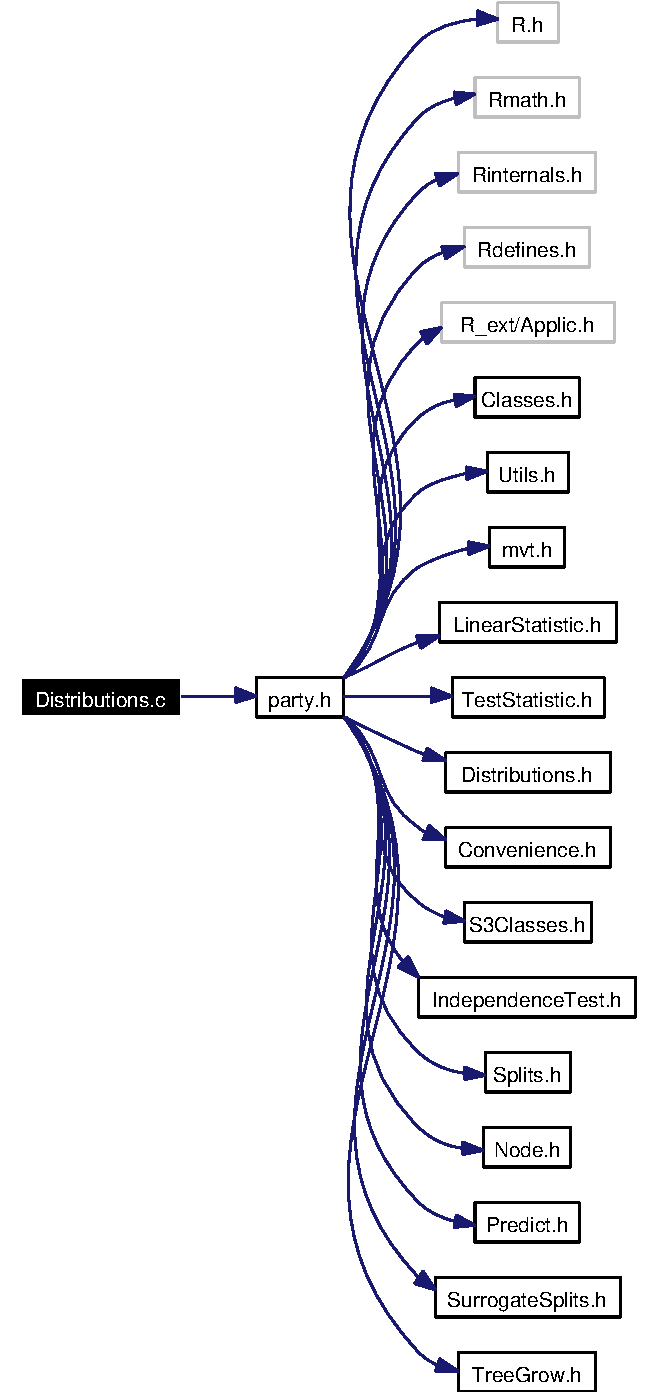
\includegraphics[width=172pt]{Distributions_8c__incl}
\end{center}
\end{figure}
\subsection*{Functions}
\begin{CompactItemize}
\item 
double \hyperlink{Distributions_8c_a0}{C\_\-quadform\-Conditional\-Pvalue} (const double tstat, const double df)
\item 
SEXP \hyperlink{Distributions_8c_a1}{R\_\-quadform\-Conditional\-Pvalue} (SEXP tstat, SEXP df)
\item 
double \hyperlink{Distributions_8c_a2}{C\_\-maxabs\-Conditional\-Pvalue} (const double tstat, const double $\ast$Sigma, const int pq, int $\ast$maxpts, double $\ast$releps, double $\ast$abseps, double $\ast$tol)
\item 
SEXP \hyperlink{Distributions_8c_a3}{R\_\-maxabs\-Conditional\-Pvalue} (SEXP tstat, SEXP Sigma, SEXP maxpts, SEXP releps, SEXP abseps, SEXP tol)
\item 
void \hyperlink{Distributions_8c_a4}{C\_\-Monte\-Carlo} (double $\ast$criterion, SEXP learnsample, SEXP weights, SEXP fitmem, SEXP varctrl, SEXP gtctrl, double $\ast$ans\_\-pvalues)
\item 
SEXP \hyperlink{Distributions_8c_a5}{R\_\-Monte\-Carlo} (SEXP criterion, SEXP learnsample, SEXP weights, SEXP fitmem, SEXP varctrl, SEXP gtctrl)
\end{CompactItemize}


\subsection{Detailed Description}
Conditional Distributions

\begin{Desc}
\item[Author:]\begin{Desc}
\item[Author]hothorn \end{Desc}
\end{Desc}
\begin{Desc}
\item[Date:]\begin{Desc}
\item[Date]2005/07/07 12:32:01 \end{Desc}
\end{Desc}


Definition in file \hyperlink{Distributions_8c-source}{Distributions.c}.

\subsection{Function Documentation}
\hypertarget{Distributions_8c_a2}{
\index{Distributions.c@{Distributions.c}!C_maxabsConditionalPvalue@{C\_\-maxabsConditionalPvalue}}
\index{C_maxabsConditionalPvalue@{C\_\-maxabsConditionalPvalue}!Distributions.c@{Distributions.c}}
\subsubsection[C\_\-maxabsConditionalPvalue]{\setlength{\rightskip}{0pt plus 5cm}double C\_\-maxabs\-Conditional\-Pvalue (const double {\em tstat}, const double $\ast$ {\em Sigma}, const int {\em pq}, int $\ast$ {\em maxpts}, double $\ast$ {\em releps}, double $\ast$ {\em abseps}, double $\ast$ {\em tol})}}
\label{Distributions_8c_a2}


Conditional asymptotic P-value of a maxabs-type test statistic\par
 Basically the functionality from package `mvtnorm' \par
 \begin{Desc}
\item[Parameters:]
\begin{description}
\item[{\em tstat}]test statitstic \item[{\em Sigma}]covariance matrix \item[{\em pq}]nrow(Sigma) \item[{\em maxpts}]number of Monte-Carlo steps \item[{\em releps}]relative error \item[{\em abseps}]absolute error \item[{\em tol}]tolerance \end{description}
\end{Desc}


Definition at line 52 of file Distributions.c.

References mvtdst.

Referenced by C\_\-Conditional\-Pvalue(), and R\_\-maxabs\-Conditional\-Pvalue().\hypertarget{Distributions_8c_a4}{
\index{Distributions.c@{Distributions.c}!C_MonteCarlo@{C\_\-MonteCarlo}}
\index{C_MonteCarlo@{C\_\-MonteCarlo}!Distributions.c@{Distributions.c}}
\subsubsection[C\_\-MonteCarlo]{\setlength{\rightskip}{0pt plus 5cm}void C\_\-Monte\-Carlo (double $\ast$ {\em criterion}, SEXP {\em learnsample}, SEXP {\em weights}, SEXP {\em fitmem}, SEXP {\em varctrl}, SEXP {\em gtctrl}, double $\ast$ {\em ans\_\-pvalues})}}
\label{Distributions_8c_a4}


Monte-Carlo approximation to the conditional pvalues \begin{Desc}
\item[Parameters:]
\begin{description}
\item[{\em criterion}]vector of node criteria for each input \item[{\em learnsample}]an object of class `Learning\-Sample' \item[{\em weights}]case weights \item[{\em fitmem}]an object of class `Tree\-Fit\-Memory' \item[{\em varctrl}]an object of class `Variable\-Control' \item[{\em gtctrl}]an object of class `Global\-Test\-Control' \item[{\em ans\_\-pvalues}]return values; vector of adjusted pvalues \end{description}
\end{Desc}


Definition at line 169 of file Distributions.c.

References C\_\-Linear\-Statistic(), C\_\-max(), C\_\-MLinear\-Statistic(), C\_\-Permuted\-Linear\-Statistic(), C\_\-Sample\-No\-Replace(), C\_\-Teststat\-Criterion(), get\_\-Mscorematrix(), get\_\-ninputs(), get\_\-nobs(), get\_\-nresample(), get\_\-transformation(), get\_\-varmemory(), get\_\-var\-Mmemory(), has\_\-missings(), is\_\-ordinal(), ncol(), PL2\_\-expcovinf\-Sym, PL2\_\-inputs\-Sym, PL2\_\-linearstatistic\-Sym, PL2\_\-responses\-Sym, and PL2\_\-sumweights\-Sym.

Referenced by C\_\-Global\-Test(), and R\_\-Monte\-Carlo().

Here is the call graph for this function:\begin{figure}[H]
\begin{center}
\leavevmode
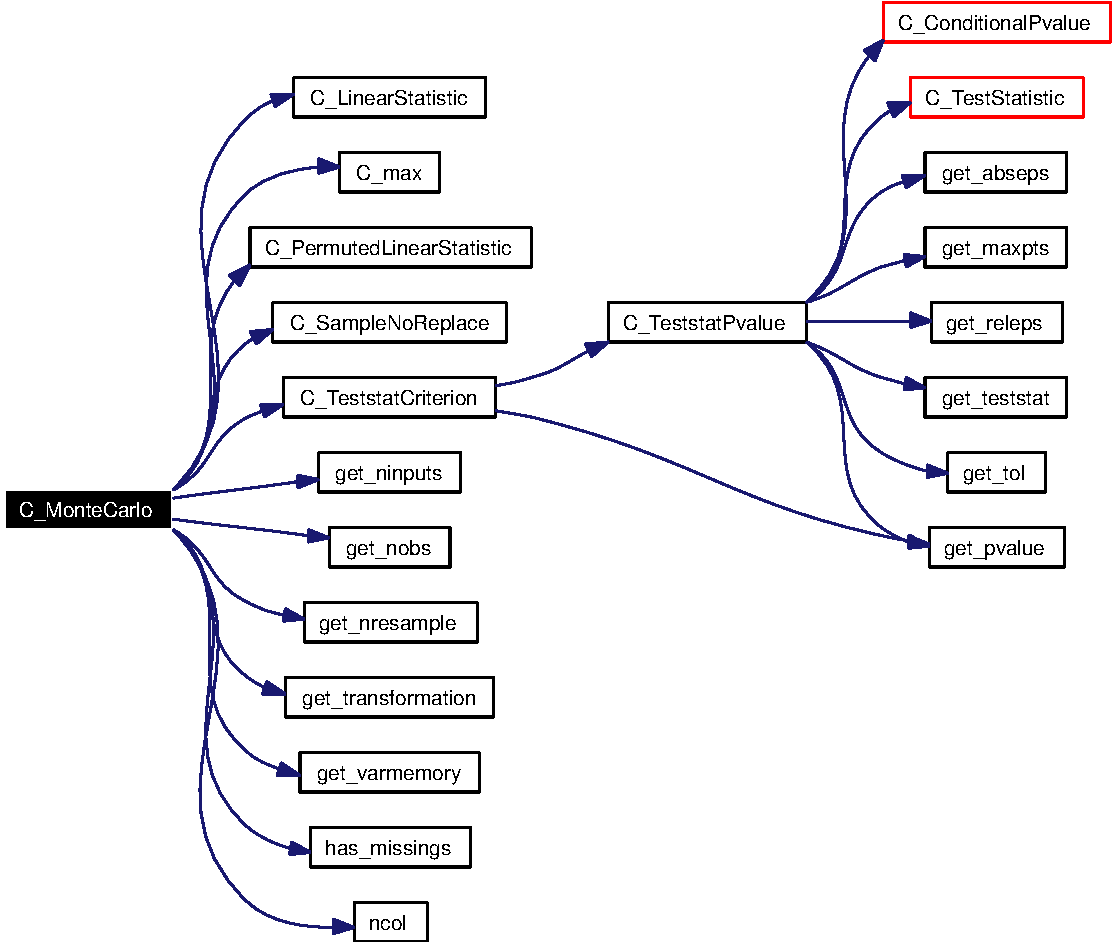
\includegraphics[width=343pt]{Distributions_8c_a4_cgraph}
\end{center}
\end{figure}
\hypertarget{Distributions_8c_a0}{
\index{Distributions.c@{Distributions.c}!C_quadformConditionalPvalue@{C\_\-quadformConditionalPvalue}}
\index{C_quadformConditionalPvalue@{C\_\-quadformConditionalPvalue}!Distributions.c@{Distributions.c}}
\subsubsection[C\_\-quadformConditionalPvalue]{\setlength{\rightskip}{0pt plus 5cm}double C\_\-quadform\-Conditional\-Pvalue (const double {\em tstat}, const double {\em df})}}
\label{Distributions_8c_a0}


Conditional asymptotic P-value of a quadratic form\par
 \begin{Desc}
\item[Parameters:]
\begin{description}
\item[{\em tstat}]test statistic \item[{\em df}]degree of freedom \end{description}
\end{Desc}


Definition at line 18 of file Distributions.c.

Referenced by C\_\-Conditional\-Pvalue(), and R\_\-quadform\-Conditional\-Pvalue().\hypertarget{Distributions_8c_a3}{
\index{Distributions.c@{Distributions.c}!R_maxabsConditionalPvalue@{R\_\-maxabsConditionalPvalue}}
\index{R_maxabsConditionalPvalue@{R\_\-maxabsConditionalPvalue}!Distributions.c@{Distributions.c}}
\subsubsection[R\_\-maxabsConditionalPvalue]{\setlength{\rightskip}{0pt plus 5cm}SEXP R\_\-maxabs\-Conditional\-Pvalue (SEXP {\em tstat}, SEXP {\em Sigma}, SEXP {\em maxpts}, SEXP {\em releps}, SEXP {\em abseps}, SEXP {\em tol})}}
\label{Distributions_8c_a3}


R-interface to C\_\-maxabs\-Conditional\-Pvalue \par
 \begin{Desc}
\item[Parameters:]
\begin{description}
\item[{\em tstat}]test statitstic \item[{\em Sigma}]covariance matrix \item[{\em maxpts}]number of Monte-Carlo steps \item[{\em releps}]relative error \item[{\em abseps}]absolute error \item[{\em tol}]tolerance \end{description}
\end{Desc}


Definition at line 142 of file Distributions.c.

References C\_\-maxabs\-Conditional\-Pvalue(), and nrow().

Here is the call graph for this function:\begin{figure}[H]
\begin{center}
\leavevmode
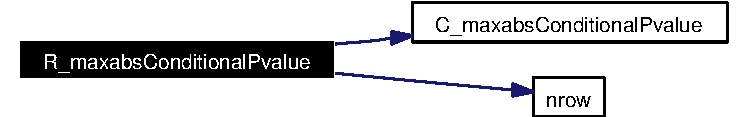
\includegraphics[width=182pt]{Distributions_8c_a3_cgraph}
\end{center}
\end{figure}
\hypertarget{Distributions_8c_a5}{
\index{Distributions.c@{Distributions.c}!R_MonteCarlo@{R\_\-MonteCarlo}}
\index{R_MonteCarlo@{R\_\-MonteCarlo}!Distributions.c@{Distributions.c}}
\subsubsection[R\_\-MonteCarlo]{\setlength{\rightskip}{0pt plus 5cm}SEXP R\_\-Monte\-Carlo (SEXP {\em criterion}, SEXP {\em learnsample}, SEXP {\em weights}, SEXP {\em fitmem}, SEXP {\em varctrl}, SEXP {\em gtctrl})}}
\label{Distributions_8c_a5}


R-interface to C\_\-Monte\-Carlo \par
 \begin{Desc}
\item[Parameters:]
\begin{description}
\item[{\em criterion}]vector of node criteria for each input \item[{\em learnsample}]an object of class `Learning\-Sample' \item[{\em weights}]case weights \item[{\em fitmem}]an object of class `Tree\-Fit\-Memory' \item[{\em varctrl}]an object of class `Variable\-Control' \item[{\em gtctrl}]an object of class `Global\-Test\-Control' \end{description}
\end{Desc}


Definition at line 289 of file Distributions.c.

References C\_\-Monte\-Carlo(), and get\_\-ninputs().

Here is the call graph for this function:\begin{figure}[H]
\begin{center}
\leavevmode
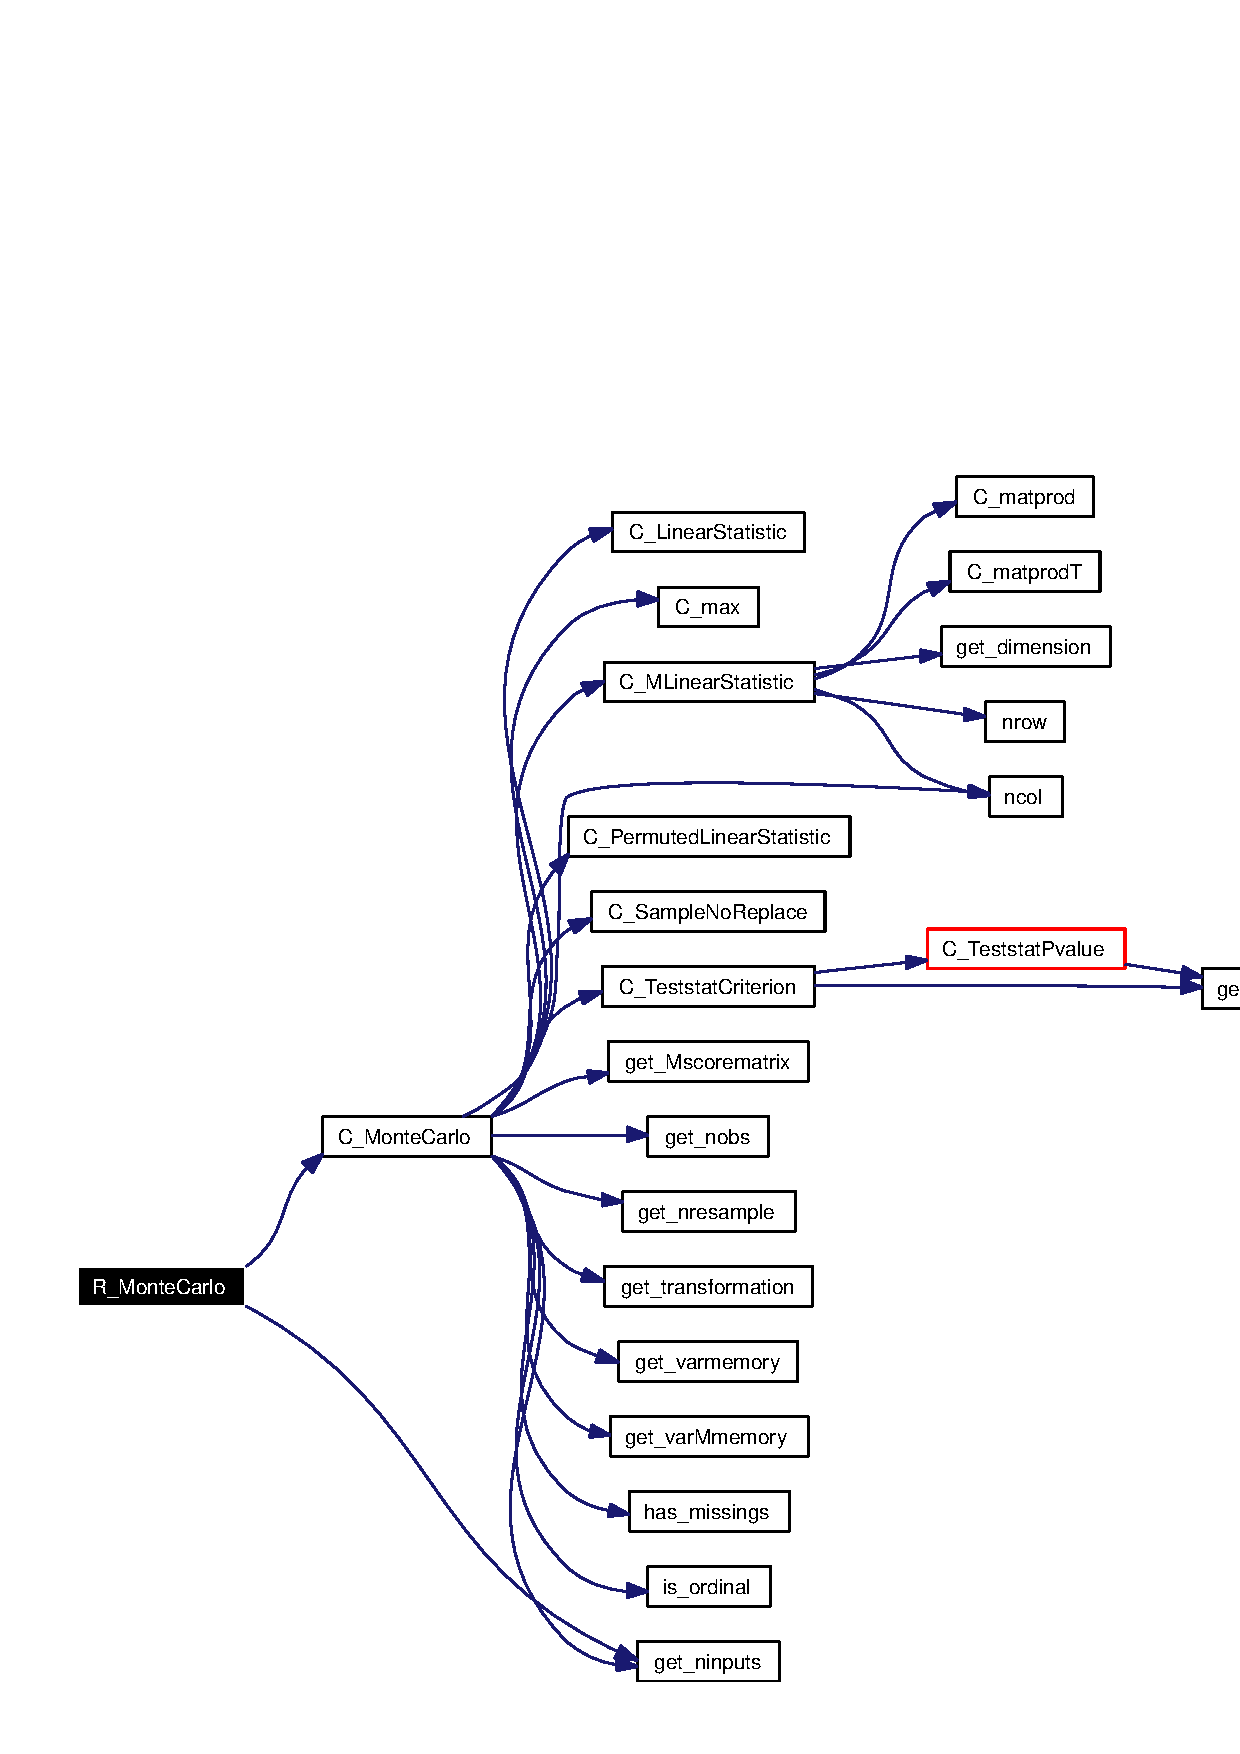
\includegraphics[width=321pt]{Distributions_8c_a5_cgraph}
\end{center}
\end{figure}
\hypertarget{Distributions_8c_a1}{
\index{Distributions.c@{Distributions.c}!R_quadformConditionalPvalue@{R\_\-quadformConditionalPvalue}}
\index{R_quadformConditionalPvalue@{R\_\-quadformConditionalPvalue}!Distributions.c@{Distributions.c}}
\subsubsection[R\_\-quadformConditionalPvalue]{\setlength{\rightskip}{0pt plus 5cm}SEXP R\_\-quadform\-Conditional\-Pvalue (SEXP {\em tstat}, SEXP {\em df})}}
\label{Distributions_8c_a1}


R-interface to C\_\-quadform\-Conditional\-Pvalue\par
 \begin{Desc}
\item[Parameters:]
\begin{description}
\item[{\em tstat}]test statitstic \item[{\em df}]degree of freedom \end{description}
\end{Desc}


Definition at line 29 of file Distributions.c.

References C\_\-quadform\-Conditional\-Pvalue().

Here is the call graph for this function:\begin{figure}[H]
\begin{center}
\leavevmode

\includegraphics[width=188pt]{Distributions_8c_a1_cgraph}
\end{center}
\end{figure}
